\section{Une méthode Agile ?}

\begin{frame}{Genèse}{Développement d’alternatives « légères »}
    \begin{tabular}{llr}
        \tabtitle{Nom de la méthode} & \tabtitle{Auteur} & \tabtitle{Année}\\
        \toprule
        Rapid Application Development & James Martin & 1991\\
        \midrule
        Dynamic Systems Development Method & --- & 1994\\
        \midrule
        \textbf{Scrum} & \textbf{Ken Schwaber} & \textbf{1995}\\
        \midrule
        Crystal Clear & Alistair Cockburn & 1996\\
        \midrule
        Extreme Programming & Kent Beck & 1996\\
        \bottomrule
    \end{tabular}
\end{frame}

\newcommand*{\itemdate}{\raisebox{-0.2\height}{
\includegraphics[height=.5cm]{icon-date}}}
\newcommand*{\itemplace}{\raisebox{-0.2\height}{
\includegraphics[height=.5cm]{icon-place}}}
\newcommand*{\itemgoal}{\raisebox{-0.2\height}{
\includegraphics[height=.5cm]{icon-target}}}

\begin{frame}{Genèse}{Réunion pour les méthodes « légères »}
    17 représentants des méthodes « légères » se réunissent.

    \vspace{1em}
    \begin{itemize}
        \item[\itemdate] \textbf{Date :} février 2001, pendant 2 jours.
        \item[\itemplace] \textbf{Lieu :} station de ski de l'Utah aux États-Unis.
        \item[\itemgoal] \textbf{Objectif :} discuter de leur expérience, mettre en commun leurs idées.
    \end{itemize}
\end{frame}

{
    \usebackgroundtemplate{%
        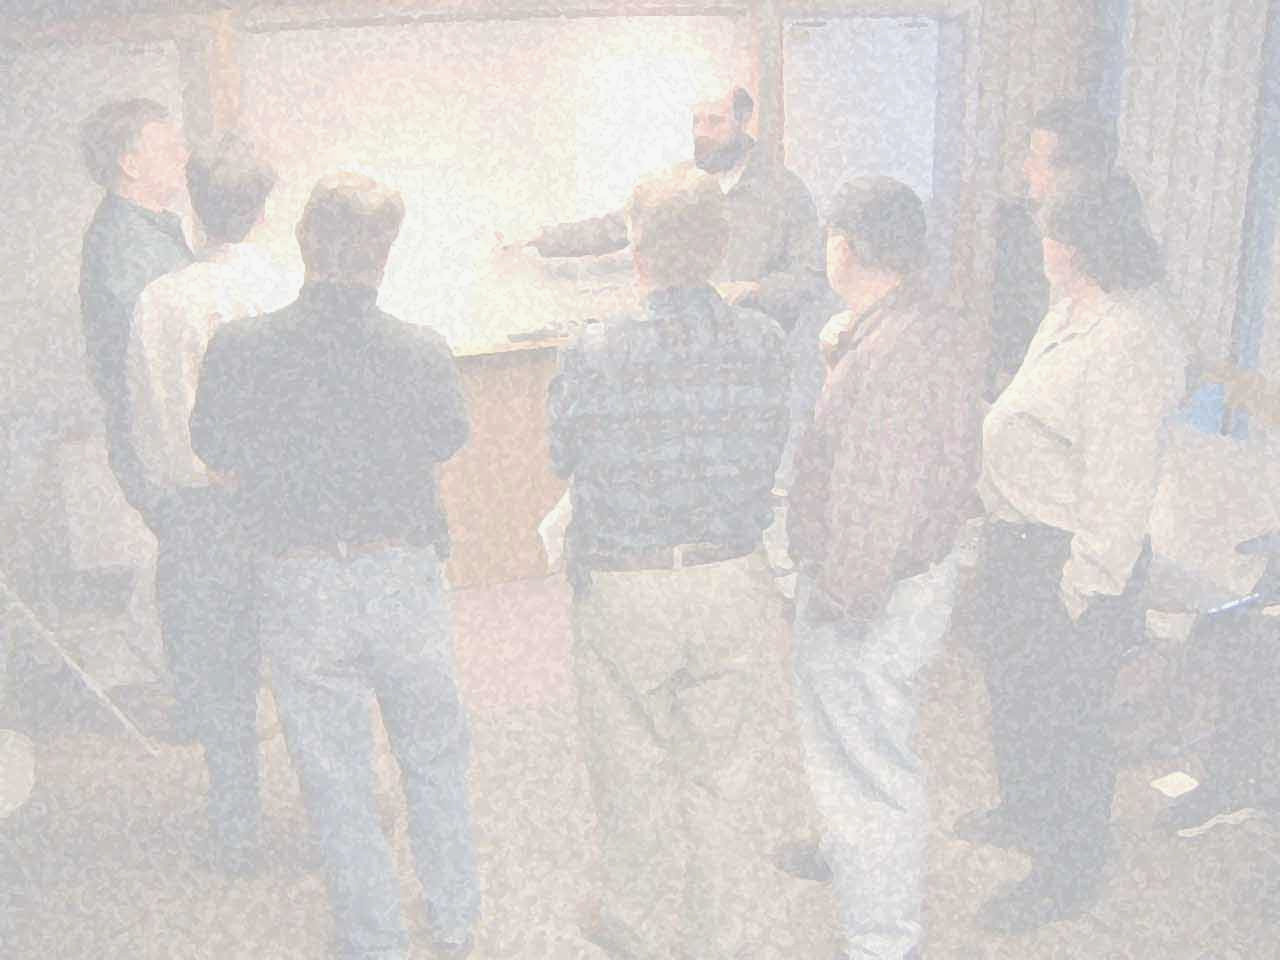
\includegraphics[width=\paperwidth]{manifeste}%
    }

    \begin{frame}{Manifeste Agile}{Définition du terme « Agile »}
        Quatre valeurs fondamentales forment le socle commun des méthodes Agiles.

        \vspace{1em}
        \begin{tabular}{rcl}
            \textbf{Humains et interactions}&$\geqslant$&processus et outils\\
            \textbf{Logiciels opérationnels}&$\geqslant$&documentation exhaustive\\
            \textbf{Collaboration avec les clients}&$\geqslant$&négociation contractuelle\\
            \textbf{Adaptation au changement}&$\geqslant$&suivi d’un plan
        \end{tabular}
    \end{frame}
}

\begin{frame}{Manifeste Agile}{Conséquences et rayonnement philosophique}
    \begin{itemize}
        \item Marque la formation de l'Agile Alliance.
        \item Renforce l'unité des méthodes agiles.
        \item Place les méthodes Agiles comme alternatives crédibles.
    \end{itemize}
\end{frame}
